\chapter{Grundlagen}
\section{Internet of Things (IoT)}
Das Internet of Things ist eine Struktur, welche alle Objekte mit einer eindeutigen Identität gekennzeichnet sind. Dadurch ist die Möglichkeit gegeben, wenn die Dinge verbunden sind, dass Informationen über ein Netzwerk übermittelt werden können. Dies kann ohne Interaktion von Mensch-zu-Mensch oder Mensch-zu-Computer durchgeführt werden. Das \gls{IoT} hat sich aus dem Zusammenspiel von der drahtlosen Kommunikation, dem Internet und mit den \gls{MEMS} (Micro-Electromechanical Systems) entwickelt.

Ein "`Thing"' im \gls{IoT} kann zum Beispiel eine Boje mit eingebauten Sensoren, ein selbstfahrendes Fahrzeug, ein Mensch mit einem Herzschrittmacher oder auch ein Haustier mit einem Biochip sein. Jedes dieser Objekte kann nützliche Informationen preisgeben. Man kann durchaus sagen, dass jedes vom Menschen geschaffene Objekt ein Kandidat dazu ist. Die Voraussetzung ist, dass es sich mit einer Netzwerkadresse beschreiben lässt und es Daten mittels eines Netzwerks übertragen kann. Die Dinge im \gls{IoT} zeichnen sich durch die Fähigkeit der Maschine-zu-Maschine Kommunikation aus. Deshalb werden diese Objekte oft auch als intelligent oder smart betitelt (vgl. \cite{mr:iotdef}).

Seit Jahren wird Forschung auf diesem Gebiet getrieben, um die Informationslücke zwischen der realen und der virtuellen Welt zu vermindern. Laut dem Forbes Magazin wird es bis Ende Jahrzehnt (2020) bereits 30 Milliarden vernetzte Dinge geben (vgl. \cite{mr:iotdef}). Cisco spricht von 50 Milliarden "`Things"' im Jahre 2025 (vgl. \cite{mk:iot}).

\section{Smartwatches}
Smartwatches sind kompakte Computersysteme, welche vom Benutzer am Handgelenk getragen werden kann. Diese können viele verschiedene Funktionalitäten mit einem Gerät abdecken. Die Minicomputer sind meist mit einer oder mehreren drahtlos Technologie und verschiedenen Sensoren (Bewegungssensor, Lichtsensor, Herzfrequenzmesser) Aktoren (Bildschirm, Vibrationsmotor) ausgerüstet.\\
Diese Uhren unterstützen den Träger beim alltäglichen Leben. Sie gehören zur Gruppe der Wearables und damit zu einem essentiellen Bereich des \gls{IoT}. Die zurzeit grössten Player auf dem Markt sind Apple, mit der Apple Watch, und Google, mit den Android Wear Geräte verschiedener Hersteller.

\section{MQTT}
\gls{MQTT} wurde im Jahre 1999 von Andy Stanford-Clark (IBM) und Arlen Nipper (damals Eurotech) entwickelt um eine Ölpipeline quer durch die Wüste zu überwachen. Das Ziel war ein Protokoll zu erhalten, welches Bandbreiteneffizient ist und wenig Energie konsumiert. Dies musste erreicht werden, weil die eingesetzten Geräte über Satelliten verbunden waren. Zu dieser Zeit war dies sehr teuer.\\
Das Protokol benutzt die publish/subscribe Architektur, im Gegensatz beansprucht HTTP request/response. Publish/subscribe ist ereignisgesteuert und erlaubt, Nachrichten an den Empfänger zu pushen. Der zentrale Kommunikationspunkt ist der \gls{MQTT} Vermittler, auch \gls{MQTT} Broker genannt. Dieser hat die Verantwortung, die Mitteilung zwischen den Sendern und den richtigen Empfängern zu verteilen. Das Routing geschieht anhand von sogenannten Themen (Topics). Topics sind vergleichbar mit Ordnerstrukturen. Sie beginnen mit einem Thema und werden anhand von Slashes unterteilt in Unterthemen. Jede Nachricht beinhaltet ein Topic. Dieser dient für den Broker als Verteilschlüssel. Jeder Empfänger abonniert die gewünschten Topics und der Broker stellt ihnen die Meldungen mit dem passenden Wert zu. Das hat den Vorteil, dass Sender und Empfänger gegenseitig nicht bekannt sein müssen. Diese Architektur erlaubt eine in hohen Masse skalierbare Lösung ohne Abhängigkeiten zwischen Datenproduzent und Konsument.\\
\begin{figure}[H]
  \centering
  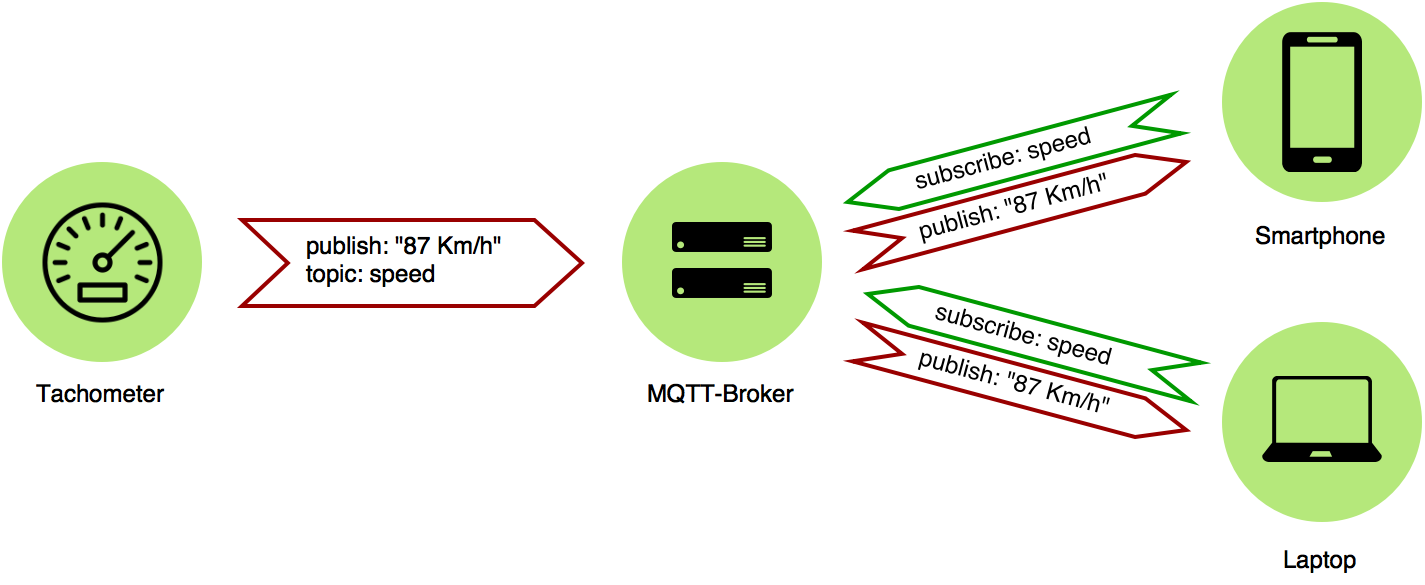
\includegraphics[scale=0.3]{98_Bilder/02_Grundlagen/MQTT}
  \caption[\gls{MQTT} Architektur]{Die Publish/Subscribe Architektur von \gls{MQTT}}
\end{figure}
Der Unterschied zum HTTP Protokoll ist, das ein dienstanforderndes Gerät die Informationen nicht holen muss, sondern direkt geliefert bekommt. Voraussetzung dafür ist eine immer offene TCP Verbindung vom Client zum Server. Falls diese Konnexion unterbrochen werden sollte, kann der \gls{MQTT} Broker Nachrichten zwischenlagern und dann pushen, wenn dieser wieder Verfügbar ist (vgl. \cite{hive:mqtt}).

\section{Node-RED}
Node-RED ist ein Open Source Tool der Firma IBM. um "`Things"', \gls{API}s und Online Services miteinander zu verbinden. Es ist ein browserbasierender Flusseditor. Es basiert auf Node.js und ist eine effiziente Applikation, um Verbindungen im \gls{IoT} zu erstellen. Es bietet auch die Möglichkeit Aktionen auszuführen, Scripts zu definieren und auch andere Online Services zu koppeln (vgl. \cite{nh:nRed}).

\section{Android und Android Wear}
Google's Android ist das marktführende Betriebssystem (vgl. \cite{stat:spos}), welches in aller Munde ist. Es betreibt Smartphones und Tablets unterschiedlicher Hersteller und ist ein Open-Source Produkt. Android Wear ist das OS von Google für Wearables, wie Smartwatches. Es basiert auf Android, ist optimiert für kleine Geräte mit weniger Leistung und kurzer Akkuausdauer.

\section{siot.net}
Die Plattform siot.net ist entstanden, um das Bedürfnis von Nutzern zu stillen, welche Geräte und Dingen ans Internet anbinden wollen, die noch nicht vernetzt sind. Im Interesse der Industriepartner, ist das Ziel diese Plattform zu industrialisieren, um Klein- und Mittlere-Unternehmen (KMU) eine Möglichkeit zu geben ihre Sensoren, Geräte, Maschinen und viele weitere Dinge zu vernetzen. Die Plattform soll ermöglichen, dass auch informatikfremde Personen und Firmen das Internet of Things nutzen können.\\
siot.net bietet ein \gls{IoT}-Center (siehe Abbildung 2.1) mit der \gls{IoT}-Infrastruktur. Konfiguration und Verwaltung werden im \gls{IoT}-Center durchgeführt. Die \gls{IoT}-Infrastruktur beinhaltet einen \gls{MQTT} Broker und das siot-Interface. Das ist die Schnittstellenspezifikation von siot.net. Nicht nach Schema angelieferte Nachrichten kann das \gls{IoT}-Center nicht interpretieren (vgl. \cite{siot:cobo}).\\
\begin{figure}[h]
  \centering
  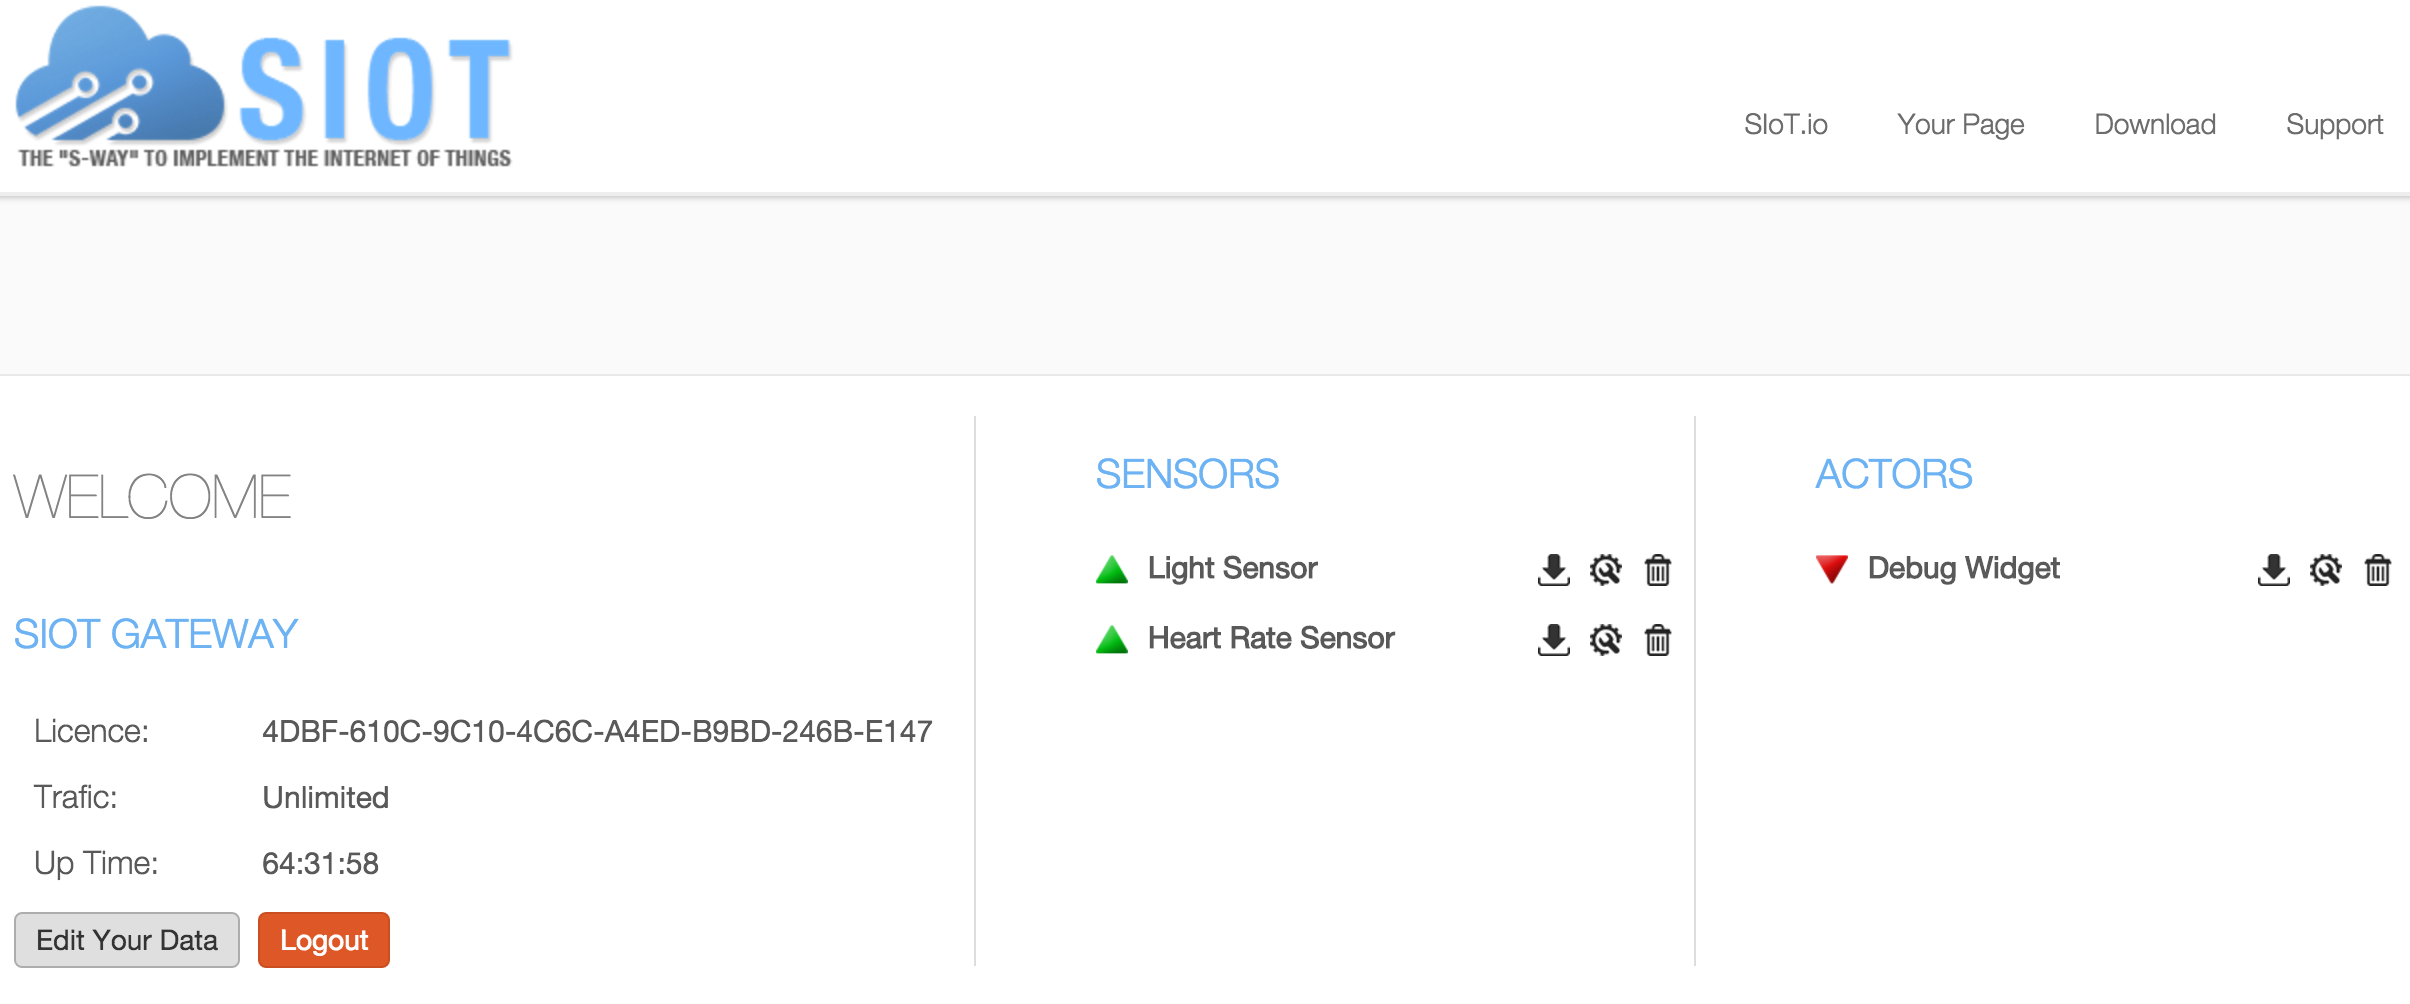
\includegraphics[scale=0.35]{98_Bilder/02_Grundlagen/siotcenter}
  \caption[siot.net IoT-Center]{siot.net \gls{IoT}-Center}
\end{figure}
\section{siot.io}
Für die Verwertung der Daten, welche die siot.net-Plattform sendet und empfängt ist das Projekt siot.io entstanden. siot.io soll die Webschnittstelle zur siot.net-Plattform implementieren. Dabei bietet sie einen Sensorsimulator, eine konfigurierbare Dashboard Applikation mit Widgets, sowie eine Node-RED Instanz für eigene Applikationen.
